
\documentclass[aps,prl,twocolumn,superscriptaddress]{revtex4-2}


\usepackage{graphicx}
\usepackage{epstopdf}
\usepackage{makecell}
\usepackage{amssymb}
\usepackage{amsmath}
\usepackage{color}
\usepackage{hyperref}
\usepackage{tikz}
\usepackage{mathrsfs}
\usepackage{wasysym}
\usepackage{tikz-cd}
\usepackage{stackengine,scalerel}
\usepackage{dblfloatfix}
\usepackage{float}

% Entorno español.
\usepackage[spanish]{babel}
\addto\captionsspanish{%
  \renewcommand{\tablename}{Tabla}%
  \renewcommand{\figurename}{Figura}%
}


\renewcommand{\thesubsection}{\thesection.\Alph{subsection}} % Produce: II.A
% Si preferís un espacio en vez de punto (II A), usá:
% \renewcommand{\thesubsection}{\thesection\ \Alph{subsection}}

% so sections, subsections, etc. become numerated.
\setcounter{secnumdepth}{3}

\DeclareMathOperator*{\argmax}{arg\,max}
\DeclareMathOperator*{\argmin}{arg\,min}
\newcommand{\avrg}[1]{\left\langle #1 \right\rangle}
\renewcommand{\appendixname}{Apéndice} % Change "Appendix" to "Apéndice"

\begin{document}

\title{
Clasificación de imágenes Fashion-MNIST con una red neuronal feedforward multicapa en PyTorch
}

\author{Bianca Abril Petry}
\email[]{bianca.petry@mi.unc.edu.ar}
\affiliation{Facultad de Psicología, Universidad Nacional de Cordoba, Boulevard de la Reforma esq. Enfermera Gordillo Gómez, Ciudad Universitaria, Córdoba, Argentina.  }

\author{Alex Ivan Wicher}
\email[]{ivan.wicher.038@mi.unc.edu.ar}
\affiliation{Facultad de Matem\'atica, Astronom\'ia, F\'isica y Computaci\'on, Universidad Nacional de C\'ordoba, Ciudad Universitaria, 5000 C\'ordoba, Argentina}

\author{Arapayu Javier Alejandro}
\email[]{arapayujavier@gmail.com}
\affiliation{Facultad de Ciencias Exactas y Naturales y Agrimensura, Universidad Nacional del Nordeste, Av. Libertad 5460, Corrientes, Argentina.}


\date{\today}

\begin{abstract}
Este informe presenta el estudio experimental de clasificación multiclase sobre el conjunto de imágenes Fashion-MNIST utilizando una red neuronal feed-forward multicapa (Perceptrón Multicapa o MLP) implementada en PyTorch. La arquitectura procesa imágenes en escala de grises de 28 x 28 píxeles aplanadas en vectores de 784 características, atravesando capas ocultas totalmente conectadas reguladas por activaciones ReLU y regularización por Dropout. El modelo fue optimizado mediante la función de pérdida de entropía cruzada (Cross Entropy Loss), comparando sistemáticamente el desempeño de los optimizadores SGD y Adam a lo largo de 30 épocas sobre una partición independiente de validación. El modelo elegido contiene los siguientes parámetros n= 128-64, Batchs= 100, Dropout= 0 y SGD-0.1. 


\end{abstract}

\maketitle

\section{Introducción}

En el ámbito del Aprendizaje Automático, las redes neuronales artificiales constituyen una herramienta fundamental para la modelización y el análisis de datos. En particular, las redes neuronales-foward multicapa representan una arquitectura muy utilizada en tareas de clasificación y regresión . Estas redes están compuestas por un conjunto de neuronas organizadas en capas, una capa de entrada, una o más capas ocultas y una capa de salida. La información fluye únicamente en un sentido desde la entrada hacia la salida, con conexiones  únicamente a la capa inmediatamente posterior. Cada neuronas realiza una combinación lineal de sus entradas seguida de la aplicación de una función de activación no lineal, lo que permite a la red aproximar funciones complejas y aprender patrones presentes en los datos.
El proceso de entrenamiento se realiza mediante el algoritmo de backpropagation, que permite calcular cómo debe ajustarse cada peso de la red a partir del error, una función de pérdida definida, cometida en la salida. Para ello se aplica la regla de la cadena a fin de obtener más derivadas parciales del error respecto a cada parámetros, y posteriormente se actualizan los pesos utilizando algún método de optimización basado en gradientes \cite{hertz1999introduction}.
En tareas de clasificación, la capa de salida se construye de modo que cada neuronas represente una posible clase, permitiendo asignar a cada entrada la etiqueta más probable según la respuesta de la red.
Una herramienta para implementar redes neuronales es en PyTorch \cite{paszke2019pytorch}, un marco de aprendizaje profundo basado en ejecución imperativa y diferenciación automática eficiente. 
El objetivo de este informe es analizar una red neuronal feed-forward multicapa mediante su desempeño en la tarea de clasificación del conjunto Fashion-MNIST.

%%%%%%%%%%%%%%%%%%%%%%%%%%%%%%%%%%%%%%%%%%%%%%%%%%%%%%%%%%%%%%%%%%%%%%%%%%%%%%%%%%%%%%%%%%%%%%%%%%%%%%%%


\section{Fundamentos y metodología}

El conjunto de datos utilizado es Fashion-MNIST, compuesto por 70.000 imágenes en escala de grises de $28 \times 28$ píxeles (valores de 0 a 255), distribuidas equitativamente en 10 categorías de prendas de vestir. Tras convertir las imágenes a tensores, los píxeles se normalizaron utilizando la media y la desviación estándar del conjunto ($\mu \approx 0.286$, $\sigma \approx 0.353$), obteniendo valores reales centrados y de módulo pequeño, adecuados para la capa de entrada en una tarea de clasificación con salidas reales no acotadas.

La arquitectura implementada es un perceptrón multicapa (MLP) compuesto por una capa de entrada de 784 neuronas, capas ocultas de menor dimensión —que actúan como cuello de botella para reducir la dimensionalidad— y una capa de salida de 10 neuronas. La cantidad y el tamaño de las capas ocultas constituyeron grados de libertad en el diseño. Cada capa oculta aplica una transformación lineal seguida de una función de activación no lineal ReLU y regularización mediante \textit{Dropout}.

La capa de salida entrega 10 valores reales sin acotar, denominados \textit{logits}, a partir de los cuales se calcula el error mediante la entropía cruzada multiclase (\texttt{nn.CrossEntropyLoss} en PyTorch). No es necesario añadir una capa \textit{Softmax} explícita al final de la red, ya que esta función opera directamente sobre los \textit{logits}: conceptualmente, los transforma internamente en una distribución de probabilidad mediante \textit{Softmax} y luego calcula el logaritmo negativo de la verosimilitud (\textit{negative log-likelihood}) de la clase verdadera, generando un escalar de pérdida que penaliza las predicciones erróneas.

\subsection{Procedimiento de entrenamiento y validación}

Para el diseño y estudio de la red se utilizó la librería PyTorch de Python. El conjunto Fashion-MNIST se dividió en entrenamiento (50.000 imágenes), validación (10.000 imágenes) y prueba (10.000 imágenes). Los dos primeros se emplearon para seleccionar los hiperparámetros óptimos: durante el entrenamiento la red ajustó sus pesos sinápticos únicamente con el conjunto de entrenamiento, mientras que en validación se evaluó el error sobre imágenes no vistas sin actualizar pesos y desactivando el \textit{Dropout} (\texttt{torch.no\_grad()} junto con \texttt{model.eval()}). Una vez seleccionada la mejor configuración, se utilizó el conjunto de prueba para reportar el desempeño final.

En cada \textit{mini-batch}, la pérdida calculada a la salida se propaga hacia atrás (\textit{backpropagation}) para obtener los gradientes respecto a cada parámetro entrenable, actualizando luego los pesos sinápticos según una tasa de aprendizaje (\textit{learning rate} . Se evaluaron dos optimizadores: SGD (\textit{Stochastic Gradient Descent}), que actualiza los parámetros en la dirección opuesta al gradiente del \textit{mini-batch} actual, y Adam (\textit{Adaptive Moment Estimation}), que mantiene estimaciones adaptativas del primer y segundo momento de los gradientes para ajustar dinámicamente la tasa de aprendizaje efectiva de cada parámetro.

\subsection{Optimización de la red MPL}

Para optimizar el MLP, se diseñaron una serie de experimentos en los cuales se exploraron distintas configuraciones (ver Tabla \ref{tab:gen}). Los modelos explorados en los experimentos se identifican por sus hiperparámetros (por ejemplo, \texttt{SGD-0.1/128-64/B100/D0} corresponde a SGD, \textit{learning rate} (LR) de 0.1, dos capas ocultas de 128 y 64 neuronas, tamaño de \textit{batch} de 100 y \textit{Dropout} de 0), fijando una duración de 30 épocas. Cada red en los experimentos fueron entrenadas y validadas de la manera descrita en la sección II.A. Se propusieron las siguientes métricas para evaluar el desempeño de las redes en cada experimento:
\begin{itemize}
    \item \textbf{Train Accuracy y Valid Accuracy:} exactitud sobre los conjuntos de entrenamiento y validación.
    \item \textbf{Worst Class Recall:} exactitud de la clase con menor desempeño en la matriz de confusión de validación en la última época.
    \item \textbf{Confusion Matrix Deviation (CM Dev.):} desviación de la matriz de confusión de validación respecto a la matriz identidad, calculada mediante la distancia de Frobenius al cuadrado.
\end{itemize}
Estas métricas se usaron como criterio de selección al comparar y elegir la mejor red en los experimentos. Como criterio ultimo de selección nos basamos en la matriz de confusión, dado que nos enfocamos no solo una alta exactitud global, sino también un desempeño equilibrado entre todas las clases.




%%%%%%%%%%%%%%%%%%%%%%%%%%%%%%%%%%%%%%%%%%%%%%%%%%%%%%%%%%%%%%%%%%%%%%%%%%%%%%%%%%%%%%%%%%%%%%%%%%%%%%%5



 \section{Resultados}
Se realizaron cinco rondas de experimentación \cite{wicher_redes_neuronales}, siendo la ultima, una evaluación con distintas semillas aleatorias. Los espacios de busqueda se detallan en la Tabla \ref{tab:gen}, donde se barrieron varias posibilidades de: Optimizador, Tamaño de Batch (mini batch), Numero de neuronas en las capas ocultas y porcentaje de Dropout.    

\begin{table}[H]
\centering
\scriptsize
\setlength{\tabcolsep}{1pt}
\begin{tabular}{c|c|c|c|c|c}
\hline
Exp. & Optimizador & Batch & Capas ocultas & Dropout & N \\
\hline
1 & \makecell{SGD/Adam\\(6 LR)} & 64,100,256,512 & (128,64) & 0.2 & 24 \\
2 & SGD-0.1 & 100 & 4 configuraciones & 0, 0.2, 0.5 & 12 \\
2B & Adam-0.001 & 512 & 4 configuraciones & 0, 0.2, 0.5 & 12 \\
3 & SGD-0.1 & 100 & (128,64) & 0,0.025,0.05,0.1 & 4 \\
Seeds & SGD-0.1 & 100 & (128,64) & 0 & 13 \\
\hline
\multicolumn{5}{r|}{Total } & 65 \\
\hline
\end{tabular}
\caption{Resumen de las configuraciones experimentales. La primera columna, Exp., declara el nombre de los experimentos, mientras que la ultima contiene el número de modelos explorados. Los 6 LR son 0.1,0.01,0.001 para SGD y 0.01,0.001,0.0001 para Adam. Las 4 configuraciones de capa oculta son (512,256), (256,128), (128,64), (64,32).}
\label{tab:gen}
\end{table}

De los 24 experimentos de la primera ronda, se seleccionaron los tres mejores que cumplen el criterio de selección (ver tabla \ref{tab:exp1}).
\begin{table}[H]
\centering
\scriptsize
\setlength{\tabcolsep}{3pt}
\begin{tabular}{c|c|c|c|c|c}
\hline
Configuración & Train Acc. & Valid Acc. & Worst Recall & CM Dev. \\
\hline
\makecell{SGD-0.1/128-64\\B100/D0.2}
& 0.909 & 0.892 & 0.713 (Shirt) & 0.245 \\

\makecell{Adam-0.001/128-64\\B512/D0.2}
& 0.915 & 0.893 & 0.700 (Shirt) & 0.241 \\

\makecell{Adam-0.001/128-64\\B256/D0.2}
& 0.914 & 0.894 & 0.668 (Shirt) & 0.262 \\
\hline
\end{tabular}
\caption{Seleccionados de ronda de experimentos 1}
\label{tab:exp1}
\end{table}

Se observa en la Tabla \ref{tab:exp2},que para capas ocultas de 512-256 volver a introducir dropout de 0.2 mejora todas las métricas respecto de su mismo tamaño sin dropout. Ademas se observa que reducir el tamaño de las capas ocultas de 128-64 a 64-32 empeora muy levemente los resultados. 

\begin{table}[H]
\centering
\scriptsize
\setlength{\tabcolsep}{3pt}
\begin{tabular}{c|c|c|c|c|c}
\hline
Configuración & Train Acc. & Valid Acc. & Worst Recall & CM Dev. \\
\hline
\makecell{SGD-0.1/128-64\\B100/D0}
& 0.941 & 0.887 & 0.781 (Coat) & 0.251 \\

\makecell{SGD-0.1/64-32\\B100/D0}
& 0.927 & 0.881 & 0.757 (Shirt) & 0.279 \\

\makecell{SGD-0.1/512-256\\B100/D0.2}
& 0.934 & 0.899 & 0.759 (Shirt) & 0.213 \\

\makecell{SGD-0.1/512-256\\B100/D0}
& 0.957 & 0.888 & 0.745 (Pullover) & 0.270 \\
\hline
\end{tabular}
\caption{Seleccionados de ronda de experimentos 2A}
\label{tab:exp2}
\end{table}

En la ronda de experimentos 2B \ref{tab:exp2B} no se observo mejora sobre el seleccionado Adam-0.001/256-128/B512/D0.2 en la ronda 1. Por lo tanto continuamos con el selccionado SGD-0.1/128-64/B100/D0 de la ronda 2A.

\begin{table}[H]
\centering
\scriptsize
\setlength{\tabcolsep}{3pt}
\begin{tabular}{c|c|c|c|c}
\hline
Configuración & Train Acc. & Valid Acc. & Worst Recall & CM Dev. \\
\hline
\makecell{Adam-0.001/256-128\\B512/D0}
& 0.955 & 0.892 & 0.633 (Shirt) & 0.275 \\

\makecell{Adam-0.001/256-128\\B512/D0.2}
& 0.931 & 0.898 & 0.730 (Shirt) & 0.225 \\

\makecell{Adam-0.001/512-256\\B512/D0.2}
& 0.941 & 0.898 & 0.715 (Shirt) & 0.233 \\

\makecell{Adam-0.001/512-256\\B512/D0.5}
& 0.904 & 0.895 & 0.673 (Shirt) & 0.248 \\
\hline
\end{tabular}
\caption{Seleccionados de ronda de experimentos 2B}
\label{tab:exp2B}
\end{table}

Como en Adam se observo anteriormente \ref{tab:exp2B} que el dropout 0.2 es optimo, o que para capas ocultas grandes re-introducir dropout mejora los resultados \ref{tab:exp2}. En la siguiente ronda de experimentos 3 se re-introdujo niveles bajos de dropout sobre SGD-0.1/128-64/B100/D0. Se observo mejora significativa en la desviación de la matriz de confusión pero a costo de perder precisión en su clase mas débil \ref{tab:exp3}.

\begin{table}[H]
\centering
\scriptsize
\setlength{\tabcolsep}{3pt}
\begin{tabular}{c|c|c|c|c}
\hline
Configuración & Train Acc. & Valid Acc. & Worst Recall & CM Dev. \\
\hline
\makecell{SGD-0.1/128-64\\B100/D0}
& 0.941 & 0.887 & 0.781 (Coat) & 0.251 \\

\makecell{SGD-0.1/128-64\\B100/D0.025}
& 0.934 & 0.888 & 0.745 (Shirt) & 0.252 \\

\makecell{SGD-0.1/128-64\\B100/D0.05}
& 0.930 & 0.889 & 0.725 (Shirt) & 0.255 \\

\makecell{SGD-0.1/128-64\\B100/D0.1}
& 0.921 & 0.890 & 0.711 (Shirt) & 0.251 \\
\hline
\end{tabular}
\caption{Seleccionados de ronda de experimentos 3}
\label{tab:exp3}
\end{table}

Se seleccionó la configuración \textbf{SGD-0.1/128-64/B100/D0}. El criterio de selección priorizó el \textit{Worst Class Recall}, con el objetivo de favorecer el reconocimiento de la clase con menor desempeño. Asimismo, se mantuvo la arquitectura de dos capas ocultas (128 y 64 neuronas), buscando un equilibrio entre la capacidad del modelo y su complejidad, sin incrementar innecesariamente su tamaño. Los tests sobre el seleccionado ademas dieron el resultado Test Loss: 0.38093.

Finalmente, se realizaron 13 ejecuciones de la configuración seleccionada, variando solo la semilla aleatoria para analizar la variabilidad y estabilidad del modelo.

Los resultados se resumen mediante la media y desviación estándar de las métricas obtenidas:

\begin{table}[H]
\centering
\small
\begin{tabular}{l|c}
\hline
\textbf{Métrica} & \textbf{Media $\pm$ Desv. Est.} \\
\hline
Train Accuracy & 0.9405 $\pm$ 0.0008 \\
Valid Accuracy & 0.8881 $\pm$ 0.0031 \\
Test Accuracy & 0.8810 $\pm$ 0.0033 \\
Valid Worst Class Recall & 0.7673 $\pm$ 0.0118 \\
TV Gap & 0.0524 $\pm$ 0.0031 \\
Valid CM Deviation & 0.2579 $\pm$ 0.0173 \\
\hline
\end{tabular}
\caption{Estadísticas de las 13 ejecuciones sobre SGD-0.1/128-64/B100/D0 con distintas semillas.}
\label{tab:seeds}
\end{table}

\begin{figure}
    \centering
    \includegraphics[width=0.88\linewidth]{TP2/figs/75matriz de confusion.png}
    \caption{Matriz de confusión normalizada del modelo seleccionado  SGD-0.1/128-64/B100/D0 sobre el conjunto de datos de tests.}
    \label{fig:fig1}
\end{figure}

\begin{figure}
    \centering
    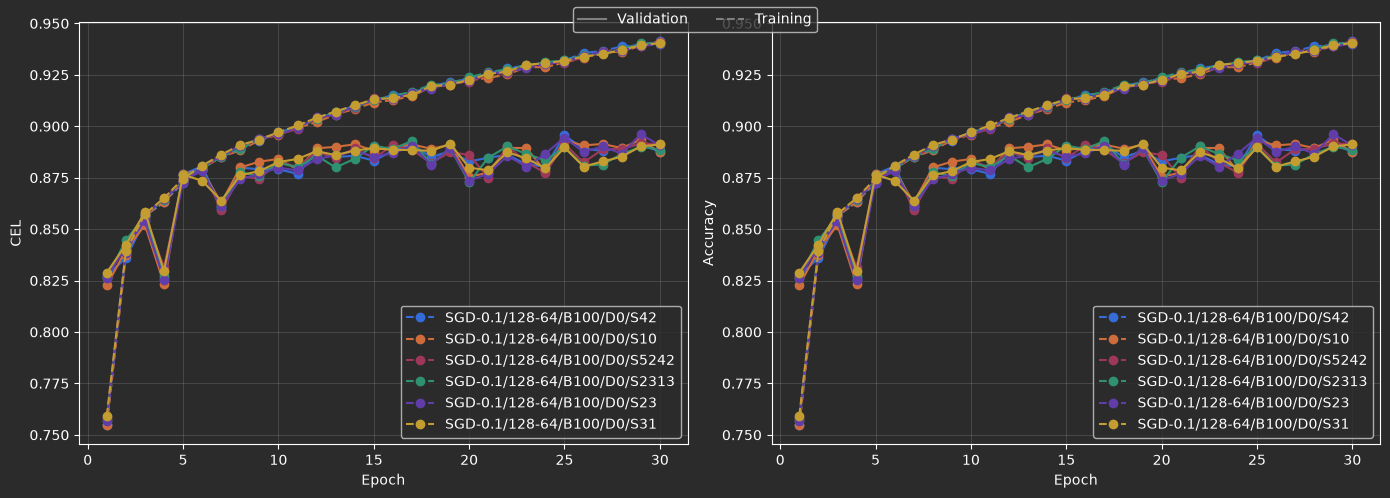
\includegraphics[width=1.0\linewidth]{figs/CurvasSeed.png}
    \caption{Curvas de perdida y precisión de SGD-
0.1/128-64/B100/D0 con 6 semillas.}
    \label{fig:fig2}
\end{figure}

\section{Discusión y conclusiones}
La configuración SGD con =0.1 (batch 100, Dropout 0.2) logró el mejor rendimiento en validación 89\% accuracy, equilibrando la clase más difícil (Shirt, 75\%) y minimizando la desviación en la matriz de confusión. La elección del optimizador depende críticamente de la tasa de aprendizaje: SGD requiere =0.1 ante la falta de momentos adaptativos, mientras que Adam rinde mejor en =0.001. Hacia la época 15–20, SGD había convergido totalmente, aplanando el costo de validación.

La variabilidad entre semillas aleatorias fue insignificante ($< 0.4\%$), confirmando que el desempeño responde a los hiperparámetros y no al azar. Las curvas muestran convergencia con sobreajuste (overfitting) moderado (entrenamiento $>94\%$ vs. validación \~88\%–89\%). Como limitación metodológica, cabe destacar que los resultados sobre el conjunto de prueba se consideraron durante la selección de hiperparámetros, lo que introduce una ligera dependencia respecto a dicho conjunto que debe contemplarse al interpretar las métricas.
\bibliography{TP2/refTP2}


\onecolumngrid



\end{document}
